\documentclass[
  bibliography=totoc,     % Literatur im Inhaltsverzeichnis
  captions=tableheading,  % Tabellenüberschriften
  titlepage=firstiscover, % Titelseite ist Deckblatt
]{scrartcl}

% Paket float verbessern
\usepackage{scrhack}

% Warnung, falls nochmal kompiliert werden muss
\usepackage[aux]{rerunfilecheck}

% unverzichtbare Mathe-Befehle
\usepackage{amsmath}
% viele Mathe-Symbole
\usepackage{amssymb}
% Erweiterungen für amsmath
\usepackage{mathtools}

% Fonteinstellungen
\usepackage{fontspec}
% Latin Modern Fonts werden automatisch geladen
% Alternativ zum Beispiel:
%\setromanfont{Libertinus Serif}
%\setsansfont{Libertinus Sans}
%\setmonofont{Libertinus Mono}

% Wenn man andere Schriftarten gesetzt hat,
% sollte man das Seiten-Layout neu berechnen lassen
\recalctypearea{}

% deutsche Spracheinstellungen
\usepackage[main=ngerman]{babel}


\usepackage[
  math-style=ISO,    % ┐
  bold-style=ISO,    % │
  sans-style=italic, % │ ISO-Standard folgen
  nabla=upright,     % │
  partial=upright,   % ┘
  warnings-off={           % ┐
    mathtools-colon,       % │ unnötige Warnungen ausschalten
    mathtools-overbracket, % │
  },                       % ┘
]{unicode-math}

% traditionelle Fonts für Mathematik
\setmathfont{Latin Modern Math}
% Alternativ zum Beispiel:
%\setmathfont{Libertinus Math}

\setmathfont{XITS Math}[range={scr, bfscr}]
\setmathfont{XITS Math}[range={cal, bfcal}, StylisticSet=1]

% Zahlen und Einheiten
\usepackage[
  locale=DE,                   % deutsche Einstellungen
  separate-uncertainty=true,   % immer Fehler mit \pm
  per-mode=symbol-or-fraction, % / in inline math, fraction in display math
]{siunitx}

% chemische Formeln
\usepackage[
  version=4,
  math-greek=default, % ┐ mit unicode-math zusammenarbeiten
  text-greek=default, % ┘
]{mhchem}

% richtige Anführungszeichen
\usepackage[autostyle]{csquotes}

% schöne Brüche im Text
\usepackage{xfrac}

% Standardplatzierung für Floats einstellen
\usepackage{float}
\floatplacement{figure}{htbp}
\floatplacement{table}{htbp}

% Floats innerhalb einer Section halten
\usepackage[
  section, % Floats innerhalb der Section halten
  below,   % unterhalb der Section aber auf der selben Seite ist ok
]{placeins}

% Seite drehen für breite Tabellen: landscape Umgebung
\usepackage{pdflscape}

% Captions schöner machen.
\usepackage[
  labelfont=bf,        % Tabelle x: Abbildung y: ist jetzt fett
  font=small,          % Schrift etwas kleiner als Dokument
  width=0.9\textwidth, % maximale Breite einer Caption schmaler
]{caption}
% subfigure, subtable, subref
\usepackage{subcaption}
%\usepackage{subfigure}


% Grafiken können eingebunden werden
\usepackage{graphicx}
\usepackage{wrapfig}
% größere Variation von Dateinamen möglich
%\usepackage{grffile}

% schöne Tabellen
\usepackage{booktabs}

% Verbesserungen am Schriftbild
\usepackage{microtype}
\setlength{\parindent}{0pt}
\setlength{\parskip}{5pt}

% Literaturverzeichnis
\usepackage[
  backend=biber,
  sorting=none
]{biblatex}
% Quellendatenbank
\addbibresource{lit.bib}
\addbibresource{programme.bib}

% Hyperlinks im Dokument
\usepackage[
  german,
  unicode,        % Unicode in PDF-Attributen erlauben
  pdfusetitle,    % Titel, Autoren und Datum als PDF-Attribute
  pdfcreator={},  % ┐ PDF-Attribute säubern
  pdfproducer={}, % ┘
]{hyperref}
% erweiterte Bookmarks im PDF
\usepackage{bookmark}

% Trennung von Wörtern mit Strichen
\usepackage[shortcuts]{extdash}

% Import PDFs
\usepackage{pdfpages}


\usepackage{graphicx}

% Chemische Notation mit Kernladung und masse
\usepackage{isotope}
% definiert Befehl \isotope[A][B]{X}
% und $\isotope[6][3]{Li}+\isotope[2][1]{H} \to\isotope[4][2]{He}+\isotope[4][2]{He}$ Beispiel






\title{Photolumineszenz von kolloidalen Nanokristallen\\
\small{FP2-Festkörperphysik}}
\author{%
  David Gutnikov\\%
  \href{mailto:david.gutnikov@tu-dortmund.de}{david.gutnikov@tu-dortmund.de} \and
  Mira Arndt\\
  \href{mailto:mira.arndt@tu-dortmund.de}{mira.arndt@tu-dortmund.de}%
}
\date{
  Abgabe: \today %??????????
}
\publishers{TU Dortmund – Fakultät Physik}
\makeatletter         
\def\@maketitle{
\raggedright
\includegraphics[width=\textwidth]{bilder/lo_TU-Do_2008/logo_rgb_jpg/tud_logo_rgb.jpg}\\[8ex]
\begin{center}
{\Huge \bfseries \sffamily \@title }\\[4ex] 
{\Large  \@author}\\[4ex] 
\@date\\[8ex]
\publishers\\
\end{center}}
\makeatother


\begin{document}


\maketitle
\thispagestyle{empty}
\tableofcontents
\newpage
%\section*{Einleitung}
Die Erfindung des \glqq scanning tunneling microscope\grqq (STM) machte erstmals die atomare Auflösung von Oberflächen möglich.
Das grundlegende Konzept beruht dabei auf der Nutzung des stark abstandsabhängigen Tunnelstroms zwischen der Probe und einer scharfen Spitze.
Eben dieses Funktionsprinzip stellt eine intrinsische Begrenzung des STM dar.
Nur metallische Oberflächen können mit dieser Methode betrachtet werden.
Das \glqq atomic force microscope\grqq (AFM) macht es möglich auch nicht-leitende Materialien aufzulösen, da hierbei die Kraft zwischen Spitze und Probe bei Distanzen von ca. $\SI{1}{nm}$ ausgenutzt wird.
Es bildet die Weiterentwicklung des STM und des stylus profilometers, wessen Auflösung durch die Größe seiner Spitze ($\sim 1\mu m$) begrenzt ist.
Ein weiterer gravierender Vorteil gegenüber dem STM besteht beim AFM darin, dass es auch an der Luft und bei Raumtemperatur bedient werden kann.
Vor diesem Hintergrund wurden in diesem Experiment mehrere Proben vermessen, um die Leistungskraft dieses Verfahrens bei der Untersuchung ihrer Topographien aufzuzeigen.

\section{Theorie}
\subsection{Kraft zwischen Spitze und Probe}
    Bei einem Spitzen-Proben Abstand von $> \SI{1}{nm}$ stellen die attraktiven langreichweitigen Kräfte, die unter der Van-der-Waals-Wechselwirkung zusammengefasst werden können, die größte Kraft dar. Diese beruhen jeweils auf der Coulomb-Wechselwirkung.
    \hspace{3cm}
    \begin{description}
        \item[Dipol-Dipol-WW:]  Diese Kraft bildet sich zwischen zwei permanent polaren Molekülen aus, die einander anziehen.
        \item[Induktions-WW:]  Kraft zwischen polarem und neutralem Molekül, wobei das Polare dem Neutralen ein magnetisches Dipolmoment induziert.
        \item[London-Dispersions-WW:]  Diese Kraft wirkt zwischen zwei neutralen Molekülen. Durch Fluktuationen entstehen spontane elektrische Dipole, die sich gegenseitig anziehen.
    \end{description}
    Die letzte überwiegt meist gegenüber den anderen beiden Kräften. \\
    Unter der Annahme zweier Edelgsatome lässt sich ihr Wechselwirkungspotential mit der Abstandsabhängigkeit
    \begin{equation*}
        V_{\mathrm{VdW}(r)} \propto -\frac{1}{r^6}
    \end{equation*}
    ausdrücken.

    Bei einem Spitzen-Proben Abstand von $< \SI{1}{nm}$ entstehen kurzreichweitige WW aufgrund des Überlapps zwischen den elektronischen Zustandsdichten.
    Wird der Abstand in fallender Ordnung durchlaufen, so ist die Wechselwirkung erst attraktiv, da durch den Überlapp der äußeren offenen Schalen chemische Bindungen entstehen, die die Gesamtenergie minimieren. \\
    \setlength{\columnsep}{10pt}
    \begin{wrapfigure}{r}{0.4\textwidth}
        \centering\captionsetup{margin={0.5cm,-1cm}, format=plain}
        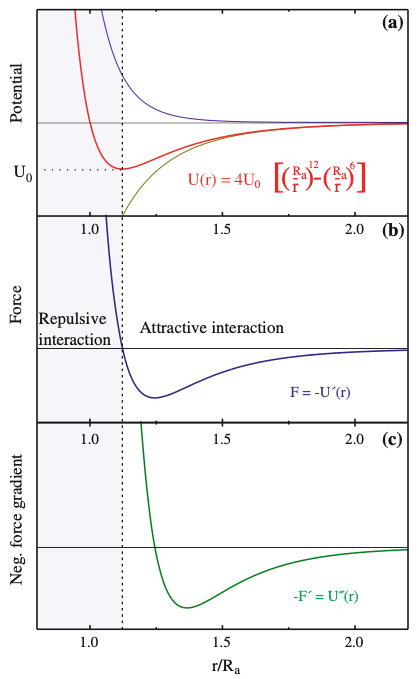
\includegraphics[width=0.48\textwidth]{bilder/Lennard_Jones_Potential.png}
        \caption{Hier ist das Lennard-Jones-Potential, seine zugehörige Kraft und dessen negierte Ableitung dargestellt.}
        \label{fig:Lennard_Jones_Potential}
    \end{wrapfigure}
    Dann kommen sich die Spitze und Probe so nah, dass die geschlossenen Orbitale überlappen.
    Die kernnahen Elektronen müssen aufgrund des Pauli-Verbotes in höhere Zustände ausweichen.
    D.h. sie müssen effektiv weiter vom Kern des anderen, an der Wechselwirkung beteiligten, Atoms entfernt sein.
    Diese Wechselwirkung wird durch
    \begin{equation*}
        V_{\mathrm{Pauli}(r)} \propto \frac{1}{r^{12}}
    \end{equation*}
    beschrieben.
    Die gesamte Wechselwirkung zwischen Sptize und Probe lässt sich also in erster Näherung durch das Lennard-Jones-Potential
    \begin{equation*}
        U(r) = 4 U_0 \left[\left(\frac{R_a}{r}\right)^{12} - \left(\frac{R_a}{r}\right)^6\right]
    \end{equation*}
    schreiben, wobei $U_0$ die Tiefe des Potentialminimums ist und $R_a$ der Abstand ist, bei dem $V(r) = 0$ gilt.
    Im obersten Graphen in \autoref{fig:Lennard_Jones_Potential} ist das Potential mit den soeben beschriebenen Parametern zu erkennen.
    Die gestrichelte Linie grenzt den repulsiven von dem attraktiven Effekt der Wechselwirkung ab.

    Eine weitere Kraft, die bei der Wechselwirkung zwischen Spitze und Probe eine große Rolle spielt, ist die elektrostatische Wechselwirkung.
    Sie entsteht durch unterschiedliche Austrittsarbeiten bzw. durch eine Ladung auf der Spitze und Probe, sodass .


\subsection{Cantilever und Spitze}

\subsection{Piezo}

\subsection{Detektion}

\subsection{Messmodi}


% \begin{figure}[ht]
%     \centering
%     \includegraphics[width=0.8\textwidth]{bilder/emission.jpg}
%     \caption{The absorption and emission processes in the active medium are shown for a two state system. \cite{anleitungHeNe}}
%     \label{fig:emission}
% \end{figure}


% \begin{figure}
%     \centering
%     \begin{subfigure}{0.49\textwidth}
%         \includegraphics[width = \textwidth]{bilder/n_Donatorschema_demtroeder.png}
%         \caption{n-doped}
%     \end{subfigure}
%     \hfill
%     \begin{subfigure}{0.49\textwidth}
%         \includegraphics[width = \textwidth]{bilder/p_Donatorschema_demtroeder.png}
%         \caption{p-doped}
%     \end{subfigure}
%     \caption{The Band structures with the fermi energy and the donor and acceptor states sre shown for p- and n-doped materials \cite{demtroeder}}
%     \label{fig:doting}
% \end{figure}

%\newpage
\section{Aufbau und Durchführung}
\subsection{Aufbau}
Ein schematisches Bild des Aufbaus ist in Abbildung \ref{fig:Aufbau} zu sehen.
\begin{figure}[H]
    \centering\captionsetup{format=plain}
    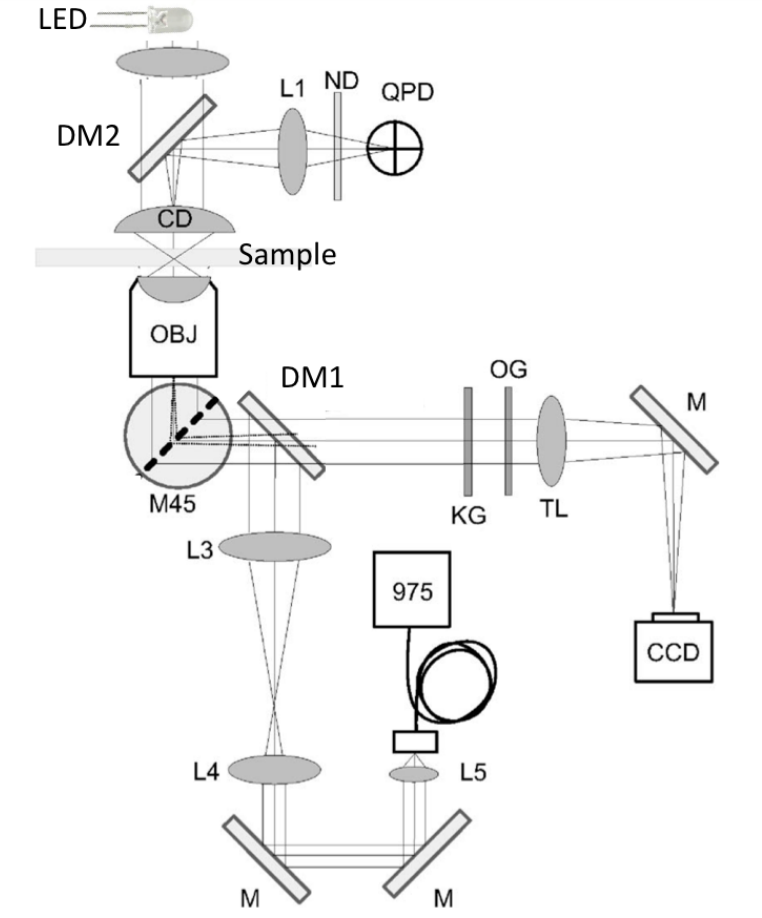
\includegraphics[width=0.7\textwidth]{Bilder/OP_Schema.png}
    \caption{Schematische Darstellung des Strahlengangs des Laserlichts durch den Aufbau der optischen Falle. Entnommen aus \cite{ref10}.}
    \label{fig:Aufbau}
\end{figure}
Dabei teilen sich die optische Pinzette und ein Mikroskop zum Beobachten der Probe 
zum Teil den Strahlengang. Das wird durch 
dichroitische Spiegel erreicht, die so arbeiten, dass sie  nur für das sichtbare Licht des
Mikroskops transparent sind und das Laserlicht im infraroten Bereich in den Strahlengang einkoppeln können.


Das Mikroskop arbeitet mit Licht im sichtbaren Bereich (Weißlicht-LED).
Dieses Licht wird über eine Linse und einen dichroitischen Spiegel fokussiert.
Über einen weiteren dichroitischen Spiegel fällt das Licht schließlich auf eine CCD Kamera.


Die optische Pinzette selbst arbeitet mit einem 975$\,$nm Laser.
Das Laserlicht wird über den gleichen dichroitischen Spiegel und ein 
Objektiv mit hoher numerischer Apertur auf die Probe fokussiert.
Detektiert wird das Signal mit einer Viersegment-Photodiode. 
Diese erlaubt neben der Bestimmung des Detektorsummensignals auch die Bestimmung der Auslenkung des Laserstrahls in x- und y-Richtung.

Die Probe befindet sich zwischen einer Kondensorlinse und einem Ölimmersionsobjektiv, bei dem ein 
Öltropfen verwendet wird um eine kontinuierlichere Änderung des Brechungsindex herbeizuführen und somit die numerische Apertur zu erhöhen.
Die Position der Probe kann mit Piezomotoren oder manuell über Mikrometerschrauben in allen drei Raumrichtungen eingestellt werden.

\subsection{Durchführung}
Zunächst soll eine Probe freier Quarzkügelchen in Wasser präpariert werden
und damit die Position der optischen Falle in den Aufnahmen der CCD-Kamera
bestimmt werden.

Mit einer Probe von fixierten Quarzkügelchen (NaCl-haltiges Wasser)
soll die Positionskalibrierung der Software in Abhängigkeit der 
Laserleistung durchgeführt werden. Die Konversionsfaktoren für die x- und y-Richtung lassen 
sich im Anschluss aus den Steigungen des linearen Bereichs der Kurven bestimmen. Außerdem soll das Diodensummensignal in Abhängigkeit des z-Piezo-Wertes 
aufgenommen werden, welches das axiale Positionssignal einer Kügelchen-Bewegung relativ zur Falle beschreibt.

Anschließend wird wieder mit freien Quarzkügelchen die Kraftkalibration der Software durchgeführt.
Zunächst ohne Krafteinwirkung in Abhängigkeit der Laserleistung und im Anschluss unter Einfluss einer oszillierenden Bewegung von außen.
Dabei soll hier in Abhängigkeit der Laserleistung untersucht werden, wann ein Kügelchen die Falle verlässt.
Abschließend soll der Einfluss eines Vortex-Retarders (ein 2$\pi$-Phasenmodulator) auf die Fallenkraft untersucht werden.

Der letzte Teil des Versuchs besteht aus dem Untersuchen von Vesikeln in Zwiebelzellen.
Dabei soll zunächst die Reaktion der Vesikel auf das Einfangen durch die optische Falle untersucht werden.
Anschließend wird der Durchmesser eines Vesikels durch Bildschirmaufnahmen bestimmt. 
Um die Geschwindigkeit zu ermitteln, wird durch die Photodiode gemessen, wie lange ein Vesikel das Laserlicht reduziert.
Zum Schluss soll untersucht werden, ab welcher Laserleistung der Aktin-Myosin-Motor die optische Falle nicht mehr überwinden kann.
\newpage
\section{Auswertung}
\label{sec:auswertung}
\subsection{Pulsdauer ohne Filter bzw. Medien}
    Als Erstes wurde der reine Laserstrahl betrachtet, ohne dass ein Filter oder ein Medium in den Strahlengang gestellt wurde.
    Dazu wurde zuerst das Spektrum in \autoref{fig:Original} (links) aufgenommen.
    Es ist ein deutliches Peak bei der zentralen Wellenlänge von $1550\,\si{\nano\meter}$ zu erkennen, doch es sind auch ein paar Neben-Peaks bei ca. 1500, 1535 und $1580\,\si{\nano\meter}$ zu sehen.
    \vspace*{-0.3cm}
    \begin{figure}[ht]
        \centering\captionsetup{format=plain}
        \includegraphics{plots/Original.pdf} \vspace*{-0.5cm}
        \caption{Links ist das Spektrum des originalen Laserstrahls dargestellt, wobei die zentrale Wellenlänge durch die grau gestrichelte Linie gekennzeichnet ist. Rechts ist die Autokorrelationsspur (blau) mit einer angepassten Summe aus Gaußglocken (rot gestrichelt) zu sehen.}
        \label{fig:Original}
    \end{figure}
    \FloatBarrier
    Die blaue Autokorrelationsspur in \autoref{fig:Original} (rechts) wird durch eine Summe von zwei Gauß-Funktionen der Formel
    \begin{equation}
        I(t) = A \cdot \exp\left(-4\ln(2)\left(\frac{t}{\Delta\tau}\right)^2\right)
    \end{equation}
    gefittet, wobei $\Delta\tau$ die Halbwertsbreite ist.
    Eine Gauß-Funktion fittet den unterliegenden zeitlich breiten Puls und eine den schmallen Peak.
    Die dabei für den Peak benutzten Werte sind mit einem breiten blauen durchsichtigen Streifen markiert und die Summe der Gaußglocken wird durch eine rot gestrichelte Linie dargestellt.
    Aus den beiden Fit-Parametern der Halbwertsbreiten der Autokorrelationsspur ergeben sich die Pulsdauern
    \begin{equation*}
        \Delta \tau_{\mathrm{orig}} \approx 70,4\,\si{\femto\second} \qquad \Delta \tau_{\mathrm{orig,breit}} \approx 205,6\,\si{\femto\second}
    \end{equation*}
    über die Formel
    \begin{equation}
        \Delta \tau_{\mathrm{Laser}} = \frac{1}{\sqrt{2}} \cdot \Delta \tau_{\mathrm{Autokorrelation}}\;.
    \end{equation}

\subsection{Pulsdauer mit Bandpassfilter}
    Anschließend wurden Messungen mit einem Bandpassfilter im Strahlengang durchgeführt.
    Das Einsetzen des $30\,\si{\nano\meter}$-Bandpassfilters ergibt ein Spektrum mit einer Halbwertsbreite von $\qty{30}{\nano\meter}$ mit nur einem prominenten Peak.
    Es ist in \autoref{fig:30nm_Bandpass} (links) jedoch noch ein leichter Neben-Peak bei $1535\,\si{\nano\meter}$ zu erkennen.
    Das liegt daran, dass dieser Neben-Peak innerhalb des $30\,\si{\nano\meter}$-Bereiches liegt und nicht ganz herausgefiltert wird.    
    \vspace*{-0.3cm}
    \begin{figure}[ht]
        \centering\captionsetup{format=plain}
        \includegraphics{plots/30nm_Bandpass.pdf} \vspace*{-0.5cm}
        \caption{Links ist das Spektrum des Laserstrahls bei Durchgang durch einen $30\,\si{\nano\meter}$-Bandpassfilter dargestellt, wobei die zentrale Wellenlänge durch die grau gestrichelte Linie gekennzeichnet ist. Rechts ist die Autokorrelationsspur (blau) mit einer angepassten Summe aus Gaußglocken (rot gestrichelt) zu sehen.}
        \label{fig:30nm_Bandpass}
    \end{figure}
    \FloatBarrier
    In \autoref{fig:30nm_Bandpass} (rechts) sind auch Schultern zu sehen und es wird wieder eine Summe aus zwei Gaußfunktionen an die Autokorrelationsspur angepasst.
    In \autoref{fig:12nm_Bandpass} (links), d.h. nach dem Einsetzen eines $12\,\si{\nano\meter}$-Bandpassfilters, ist nur noch ein scharfer Peak um die zentrale Wellenlänge zu sehen.
    Generell wird der Bereich der im Fit einbezogenen Werte so gewählt, dass die angepassten Funktionen auch den breiten Puls möglichst genau überlagern.
    Die Anpassungen ergeben die Pulsdauern:
    \begin{align*}
        \Delta \tau_{\mathrm{bandpass,30}} \approx 160,3\,\si{\femto\second} \qquad \Delta \tau_{\mathrm{bandpass,30,breit}} \approx 532,8\,\si{\femto\second} \\
        \Delta \tau_{\mathrm{bandpass,12}} \approx 268,2\,\si{\femto\second} \qquad \Delta \tau_{\mathrm{bandpass,12,breit}} \approx 579,9\,\si{\femto\second}
    \end{align*}
    \begin{figure}[ht]
        \centering\captionsetup{format=plain}\vspace*{-1cm}
        \includegraphics{plots/12nm_Bandpass.pdf} \vspace*{-0.5cm}
        \caption{Links ist das Spektrum des Laserstrahls bei Durchgang durch einen $12\,\si{\nano\meter}$-Bandpassfilter dargestellt, wobei die zentrale Wellenlänge durch die grau gestrichelte Linie gekennzeichnet ist. Rechts ist die Autokorrelationsspur (blau) mit einer angepassten Summe aus Gaußglocken (rot gestrichelt) zu sehen.}
        \label{fig:12nm_Bandpass}
    \end{figure}
    \FloatBarrier

\subsection{Pulsdauer mit dispersiven Medium}
    \begin{figure}[H]
        \centering\captionsetup{format=plain}\vspace*{-0.5cm}
        \includegraphics{plots/Si_12mm.pdf} \vspace*{-0.5cm}
        \caption{Links ist das Spektrum des Laserstrahls bei Durchgang durch einen $12\,\si{\milli\meter}$-Block Si dargestellt, wobei die zentrale Wellenlänge durch die grau gestrichelte Linie gekennzeichnet ist. Rechts ist die Autokorrelationsspur (blau) mit einer angepassten Gaußglocke (rot gestrichelt) zu sehen.}
        \label{fig:Si_12mm}
    \end{figure}
    \FloatBarrier
    Hierbei wurden verschiedene dispersive Medien in den Strahlengang eingesetzt.
    Als Erstes wurde ein $12\,\si{\nano\meter}$ dicker Block Si benutzt.
    Da hier keine Filter verwendet werden, ähnelt das Spektrum in \autoref{fig:Si_12mm} sehr dem in \autoref{fig:Original}.
    Es ist eine deutliche Verbreiterung der Autokorrelationsspur zu erkennen.
    Die zugehörige Pulsdauer ergibt sich zu
    \begin{equation*}
        \Delta \tau_{\mathrm{Si}} \approx 562,6\,\si{\femto\second}
    \end{equation*}
    Um einen möglichen Zusammenhang besser erkennen zu können, werden die Autokorrelationsspuren bei verschiedenen Glasdicken in einem Plot in \autoref{fig:Glas} zusammengefasst.
    Es wird das gleiche Verfahren angewandt, wie bei den anderen Messungen.
    \begin{figure}[t]
        \centering\captionsetup{format=plain}
        \includegraphics{plots/Glas.pdf} \vspace*{-0.5cm}
        \caption{Die Gauß-Fits der Autokorrelationsspuren bei verschiedenen Glasdicken sind hier dargestellt.}
        \label{fig:Glas}
    \end{figure}
    \FloatBarrier

    Die bestimmten Pulsdauern sind in \autoref{tab:Glas} eingetragen und es ist ein klarer Trend zu erkennen.
    Je dicker das Glas ist, desto größer ist die Pulsdauer.
    \begin{table}[h]
        \centering
        \caption{.}
        \label{tab:Glas}
        \begin{tabular}{c c}
        \toprule
        {Glasdicke [mm]} & {Pulsdauer $\Delta \tau$ [fs]}  \\
        \midrule
        \num{2.85}     &   \num{96,9\pm1,5}  \\
        \num{5.31}     &   \num{97,1\pm1,4}  \\
        \num{96,3}     &   \num{97,4\pm1,4}  \\
        \num{13,51}    &   \num{96,9\pm1,4}  \\
        \num{23,85}    &   \num{98,0\pm1,4}  \\
        \num{23,85}    &   \num{98,7\pm1,5}  \\
        \num{29,83}    &   \num{103,0\pm1,6} \\
        \bottomrule
        \end{tabular}
    \end{table}
    Als Ausdruck der Dispersion, die der Puls aufgrund des Durchgangs durch das Material erfährt, lässt sich die "group velocity dispersion" bestimmen






 \newpage
\section{Diskussion}
\label{sec:discussion}
Dieser Versuch war in dem Sinne erfolgreich, ein allgemeines Gefühl für die Maßstäbe und für die bei der Optischen Pinzette involvierten Kräfte zu vermitteln.

Die gelegentlich stark abweichenden Werte bei der Kalibrierung der Fallensteifigkeit liegen wahrscheinlich daran, dass die Kalibrierungsdauer mit $\Delta t_{\mathrm{cal}} = \qty{1}{s}$ zu niedrig eingestellt war und die Quarzkugel in ihrer Brown'schen Bewegung durch andere äußere Einflüsse gestört worden ist.

Die berechneten Boltzmannkonstanten sollten dem Überprüfen der Fallensteifigkeiten dienen und so in ungefähr der gleichen Größenordnung wie der Theoriewert liegen.
Bei der Fallensteifigkeit sind die meisten Werte in der richtigen Größenordnung und stimmen mit den Werten anderer Praktikumsgruppen grob überein.
Nach der Umrechnung in die Boltzmannkonstante sind jedoch sehr große Abweichungen zu erkennen.
Das könnte heißen, dass die Varianz der gemessenen Daten zu groß ist.

Die Stokes'sche Fallenkraft konnte aufgrund der technischen Gegebenheiten nicht bestimmt werden, denn dazu wäre das Messen der Flucht-Frequenz $f_{\mathrm{escape}}$ einer Quarzkugel erforderlich gewesen.
Die Flucht-Frequenz ist die maximale Frequenz der sinusförmigen Oszillation der Stage, bis zu der die Kugel noch von der Optischen Pinzette gehalten werden kann.
Das Problem lag daran, dass die Amplitude $A$ dieser Schwingung mit steigender Frequenz kleiner wurde und eventuell kleiner als der Durchmesser der Falle war.
Aus diesem Grund konnte die $f_{\mathrm{escape}}$ nicht mehr mit dem bloßen Auge erkannt werden, da sich die Quarzkugel immer in der Falle befand.

Die Charakterisierung der Vesikelbewegung mit Hilfe der Aktin-Myosin-Motoren in einer Zwiebelzelle ist erfolgreich verlaufen und haben zu unserem Verständnis des Vesikeltransports beigetragen.
Die Messungen der Bremskraft der Myosin-Motoren wurden dadurch erschwert, dass seit Anfang der Messungen ca. 45 Minuten vergangen sind.
Das hatte zur Folge, dass die Aktin Fasen nicht mehr leicht zu erkennen waren und die Bereiche, in denen die Vesikel transportiert wurden sich verbreitert haben.
So wurde es zunehmend schwieriger den Weg der Vesikel zum Abfangen vorauszuahnen.
Außerdem waren die Faser oft nicht parallel zur Probenoberfläche, sondern gingen auch in die Tiefe, sodass man lange nach geeigneten Faserbereichen suchen musste.

 \newpage
 \nocite{*}
 \printbibliography
 %\newpage
\section{Appendix}
\label{sec:Appendix}

Hier in den Appendix kommen eventuell die Messdaten

\end{document}